\section{Results}\label{sec:results}

    \subsection{Multi-image versus single-image super resolution}

    \subsection{Domain gap effects}

    \subsection{Domain adaptation}

        \subsubsection{Source Domain (ECOSTRESS)}

        \begin{figure}[ht!]
            \centering
            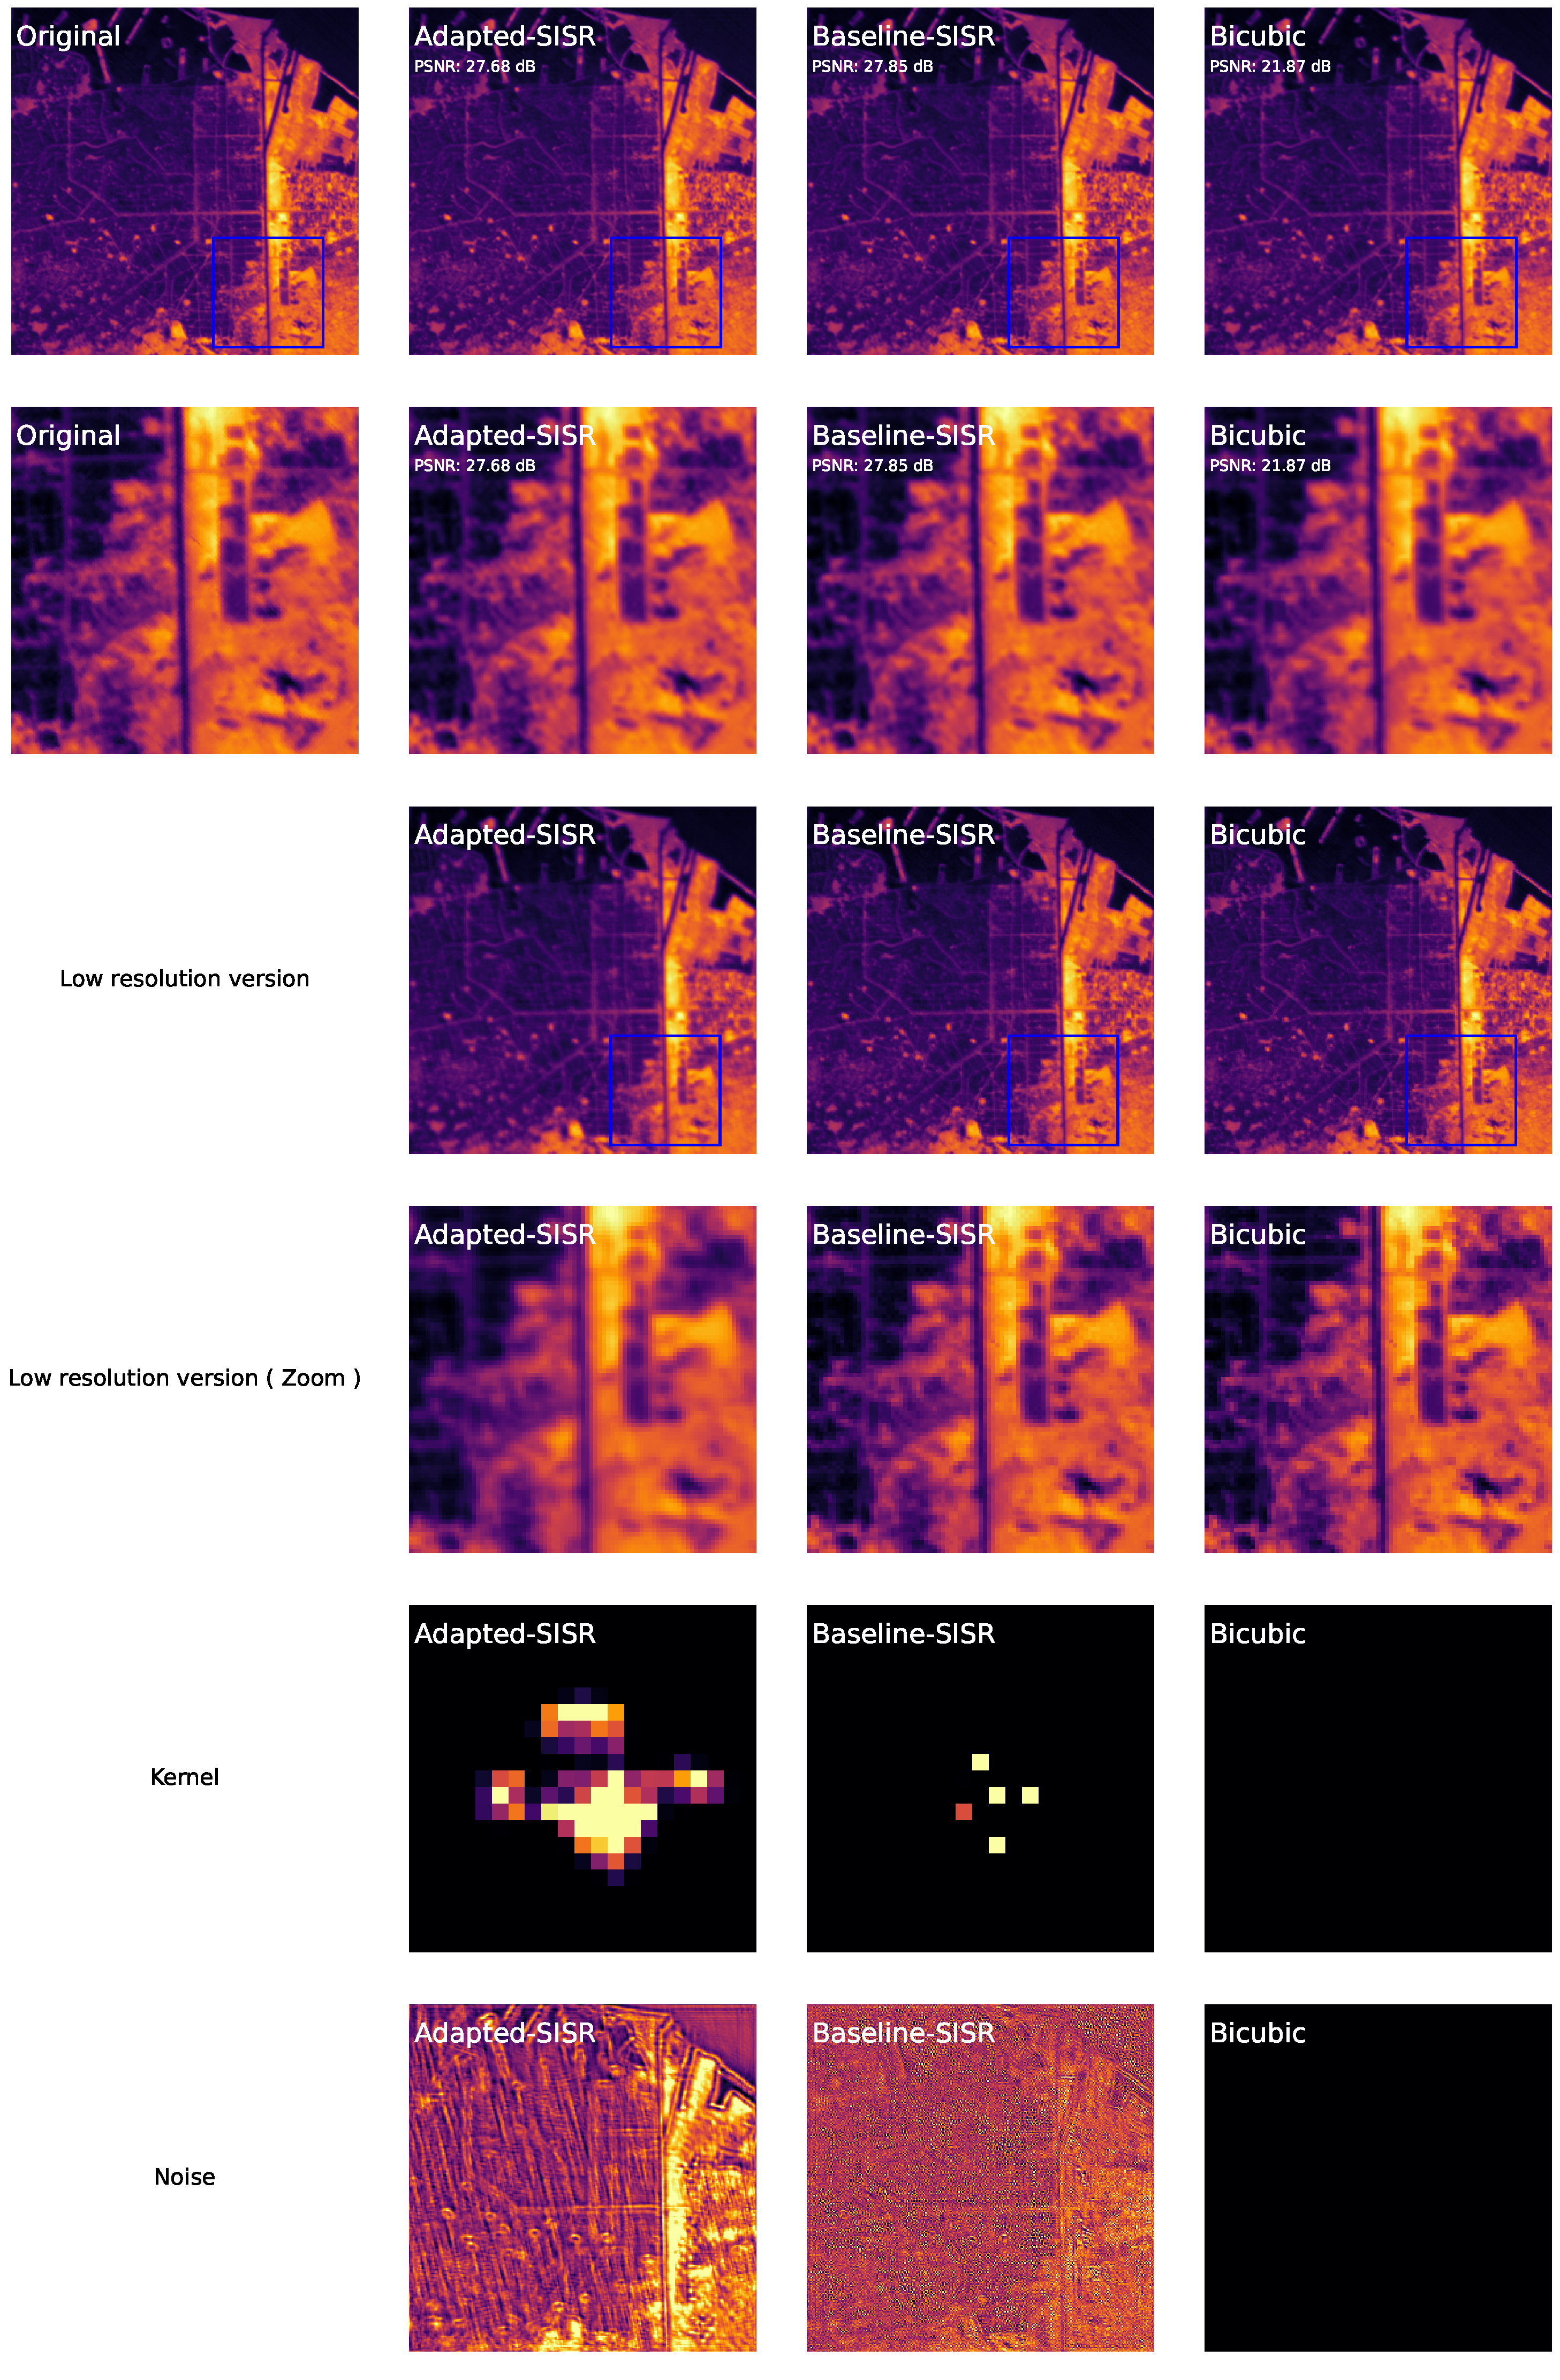
\includegraphics[scale=0.28]{Includes/6-source_prediction-sample.pdf}
            \caption{Applying different degradation models on an HR sample. In the Baseline SISR, the target domain used for training the generator is composed of ECOSTRESS images with the baseline degradation model applied.  }
            \label{fig:6-source_domain_sample}
        \end{figure}


        \begin{figure}[h!]
            \centering
            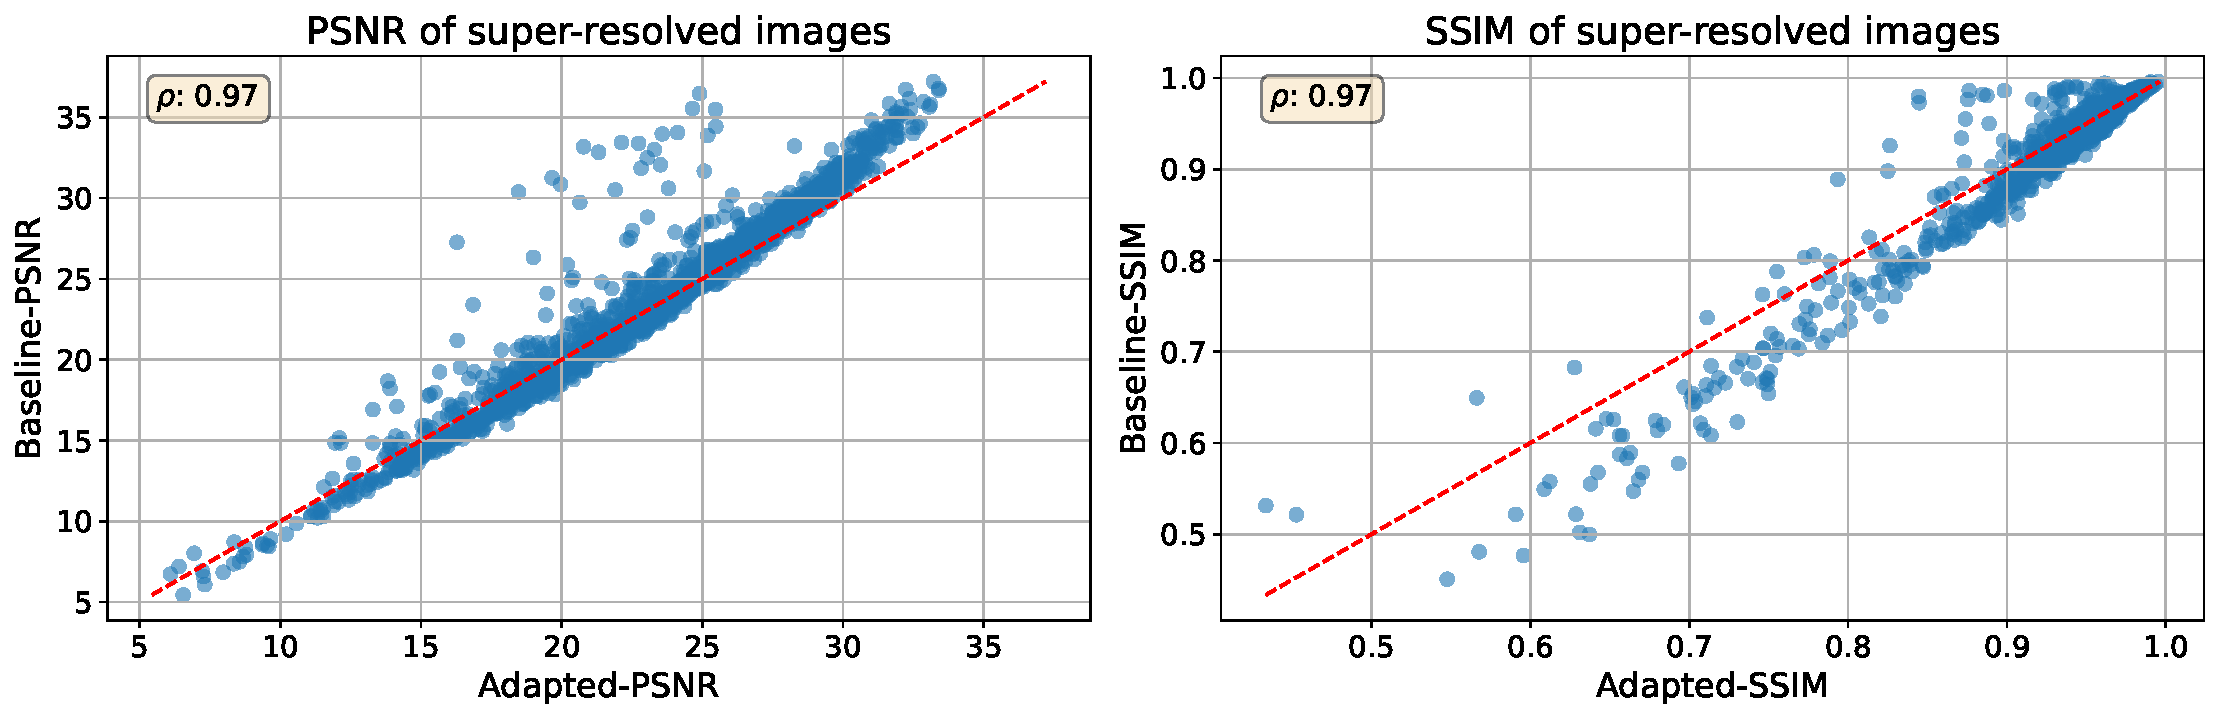
\includegraphics[width=\linewidth]{Includes/5-source-domain-sr-comparison.pdf}
            \caption{Performance obtained by using different generators to degrade the source domain and then applying the trained super resolution model .}
            \label{fig:5-source-domain-sr-comparison}
        \end{figure}


        \begin{figure}[h!]
            \centering
            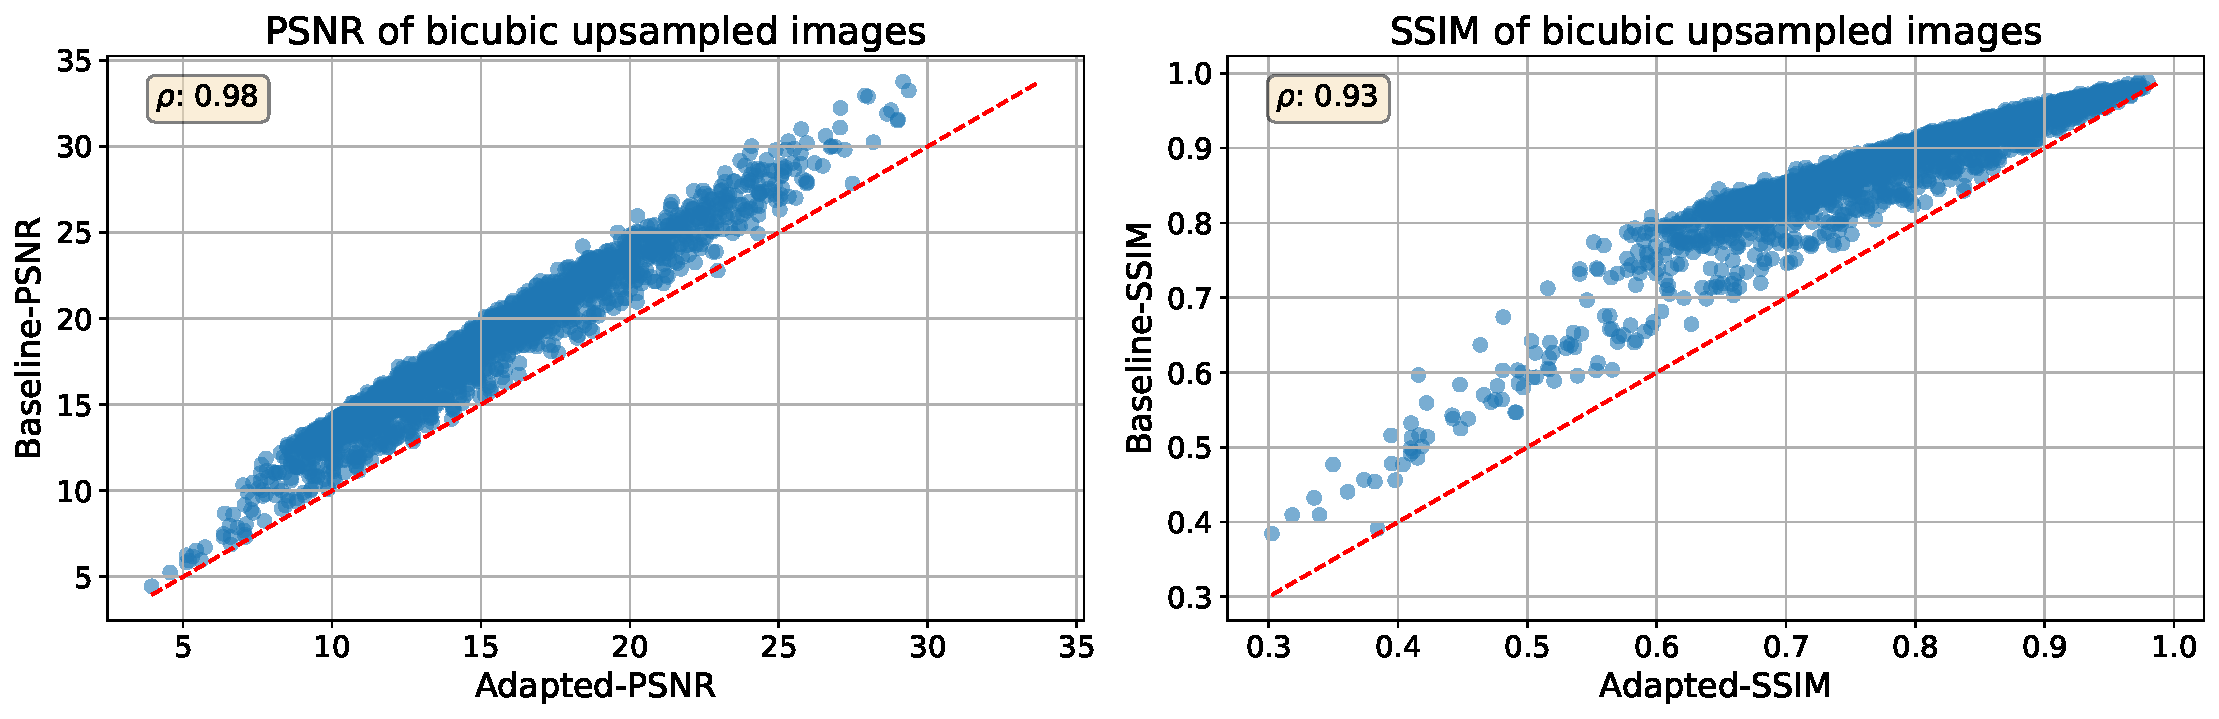
\includegraphics[width=\linewidth]{Includes/5-source-domain-bicubic-upsampling-comparison.pdf}
            \caption{Performance obtained by using different generators to degrade the source domain and then applying bicubic upsampling.}
            \label{fig:5-source-domain-bicubic-upsampling-comparison}
        \end{figure}

        \begin{figure}[h!]
            \centering
            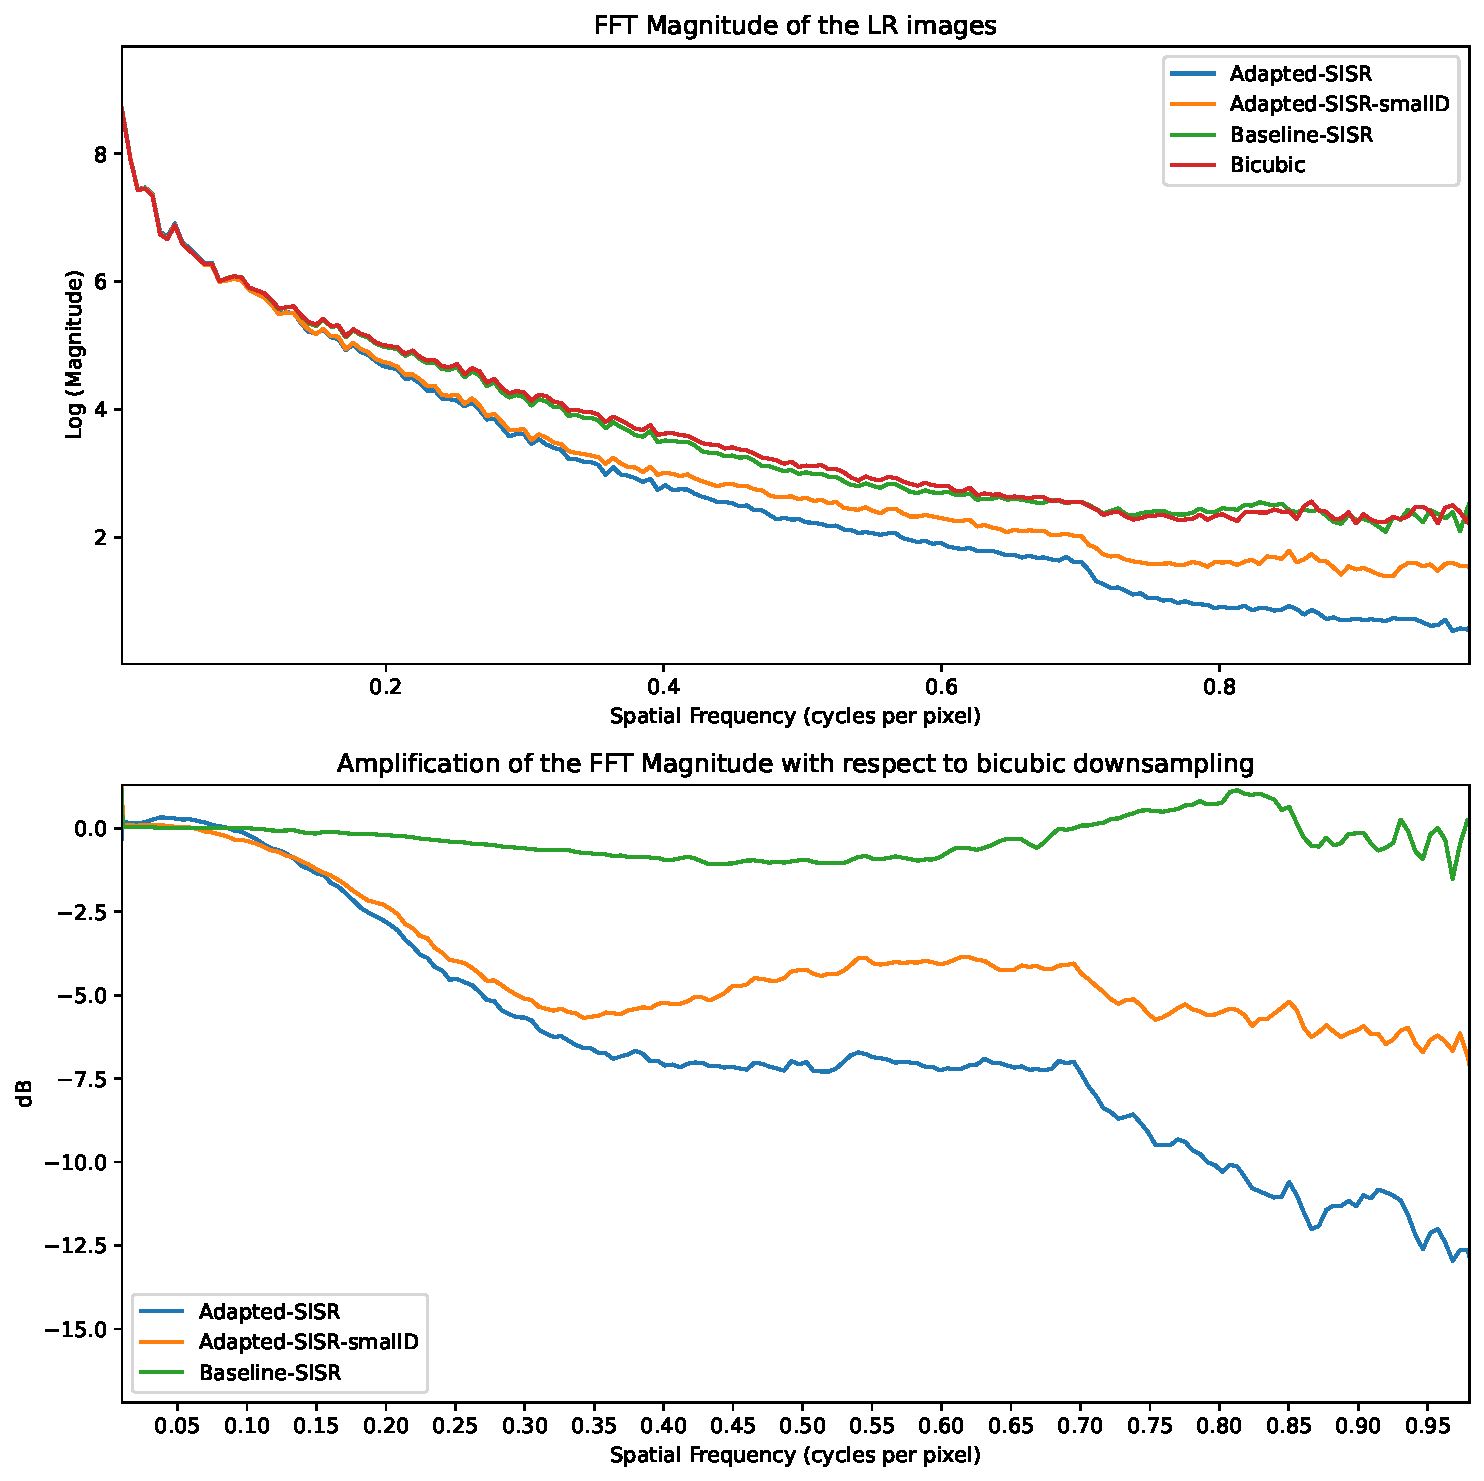
\includegraphics[scale=0.5]{Includes/6-lr-images-fft-comparison.pdf}
            \caption{Sample }
            \label{fig:6-source_domain_fft_comparison}
        \end{figure}
        
    
        \subsubsection{Target domain (FOREST)}
            \begin{figure}[ht!]
                \centering
                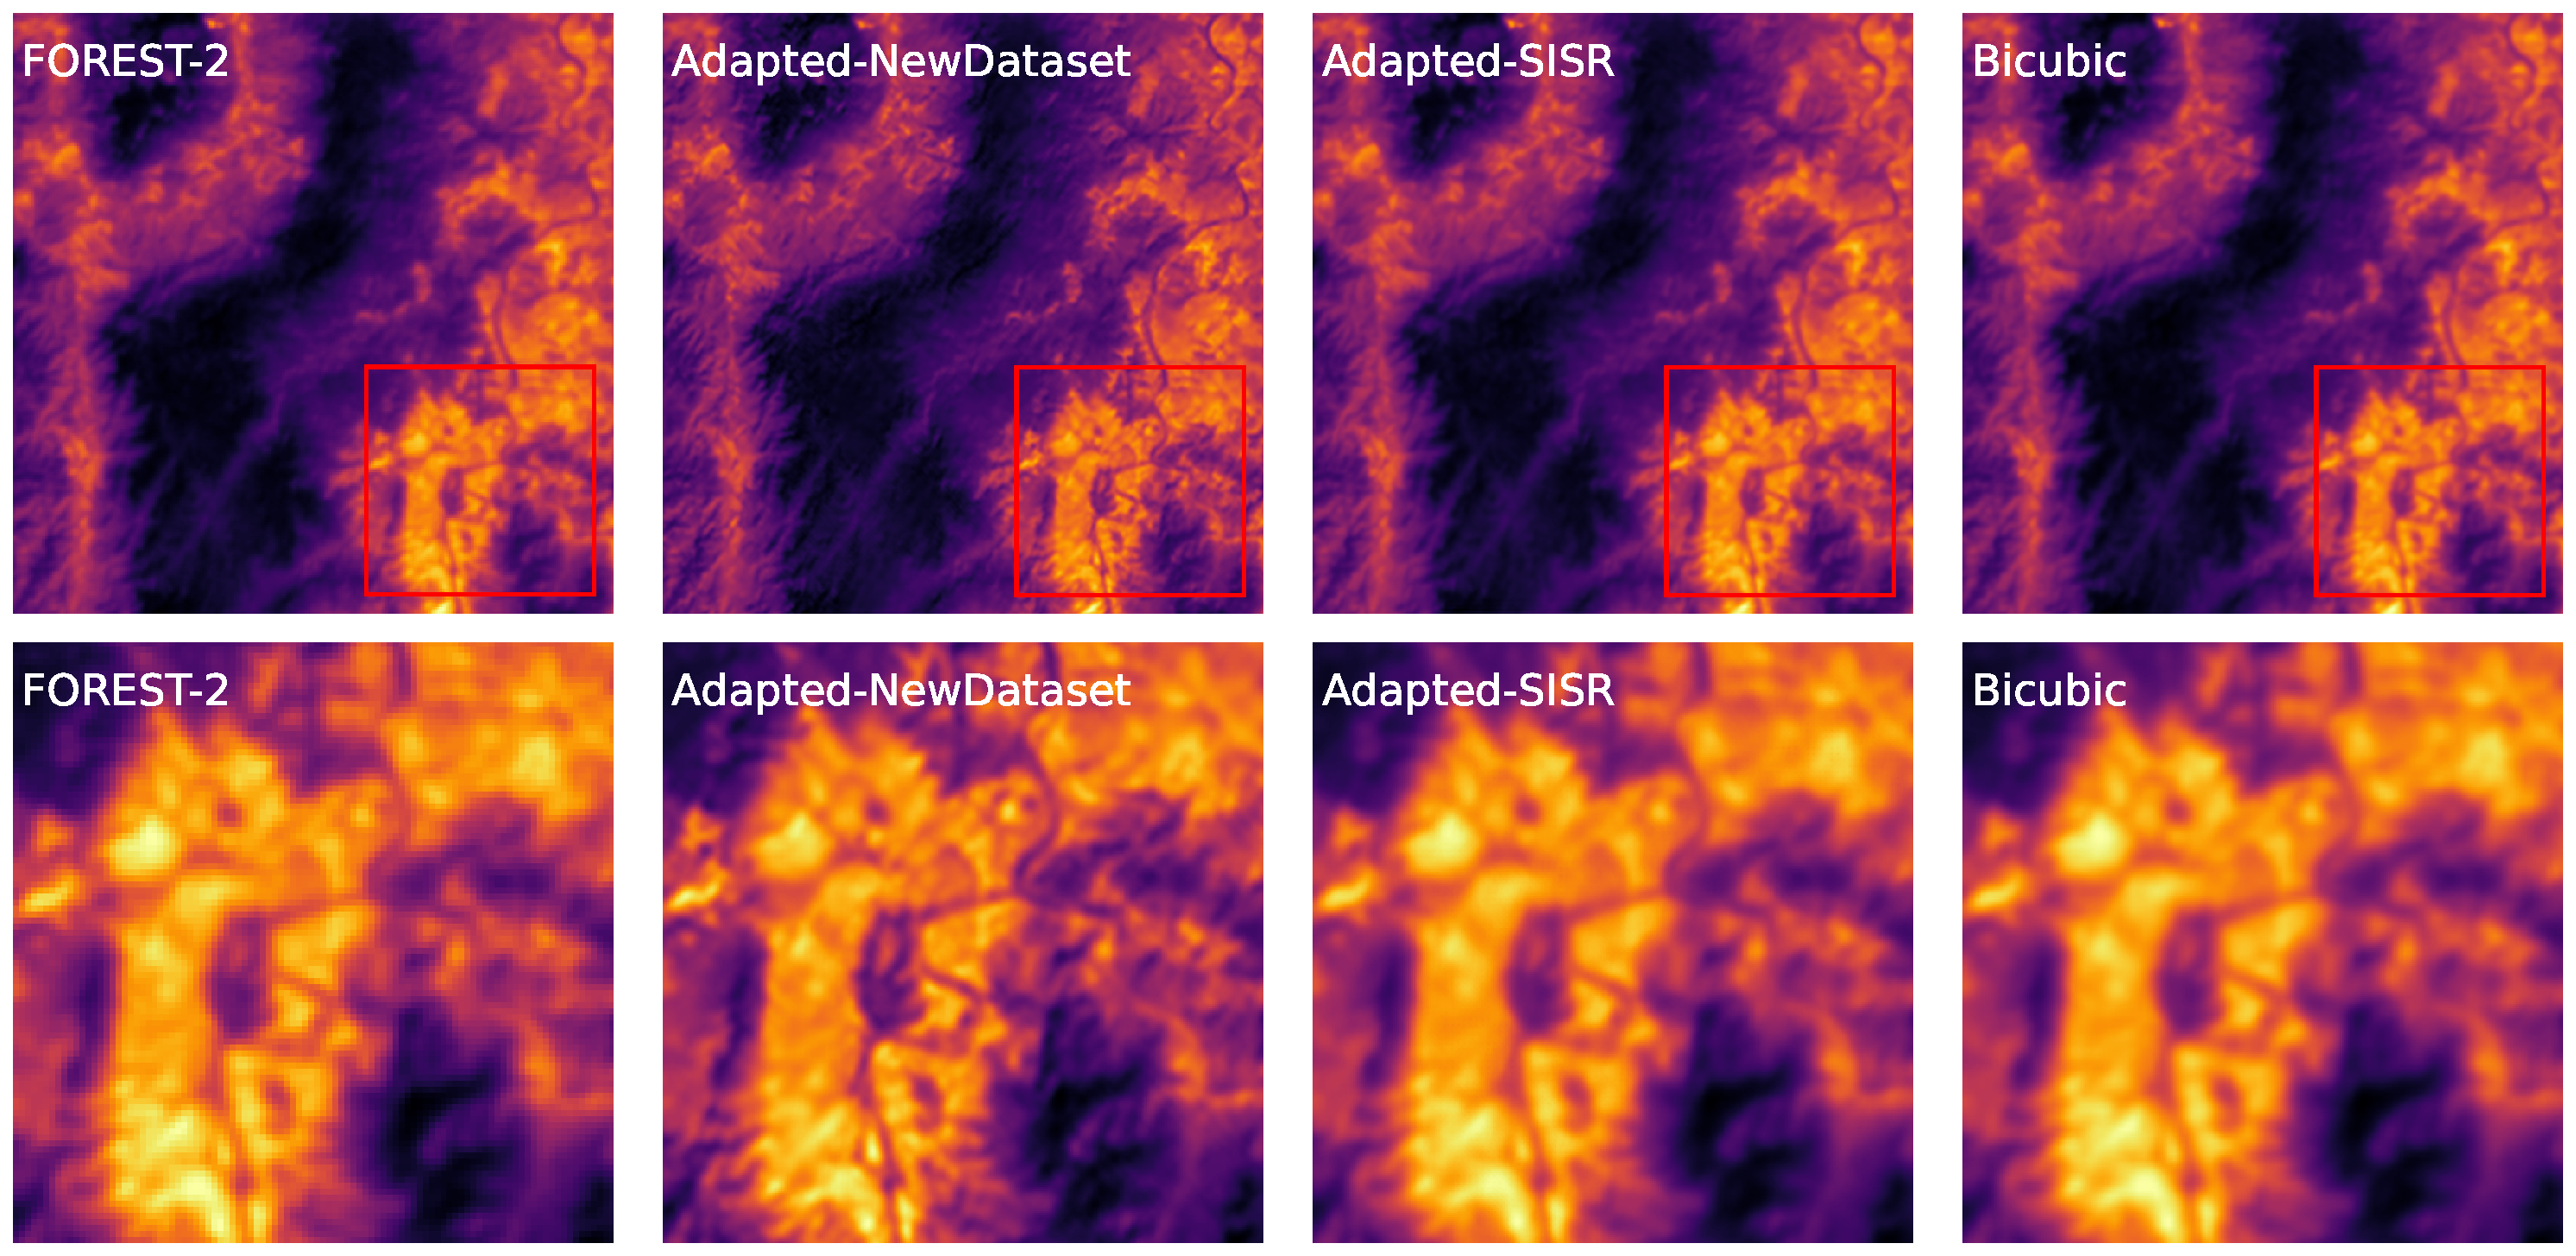
\includegraphics[scale=0.3]{Includes/6-target_prediction_sample.pdf}
                \caption{Sample of adapted SISR}
                \label{fig:6-target_prediction_sample}
            \end{figure}


            \begin{figure}[ht!]
                \centering
                \includegraphics[scale=0.3]{Includes/6-target-fft-sample.pdf}
                \caption{Super Resolved Forest-2 Scene using bicubic upsampling, the baseline blind SISR and the adapted approach.}
                \label{fig:6-target-fft-sample}
            \end{figure}


            \begin{figure}[ht!]
                \centering
                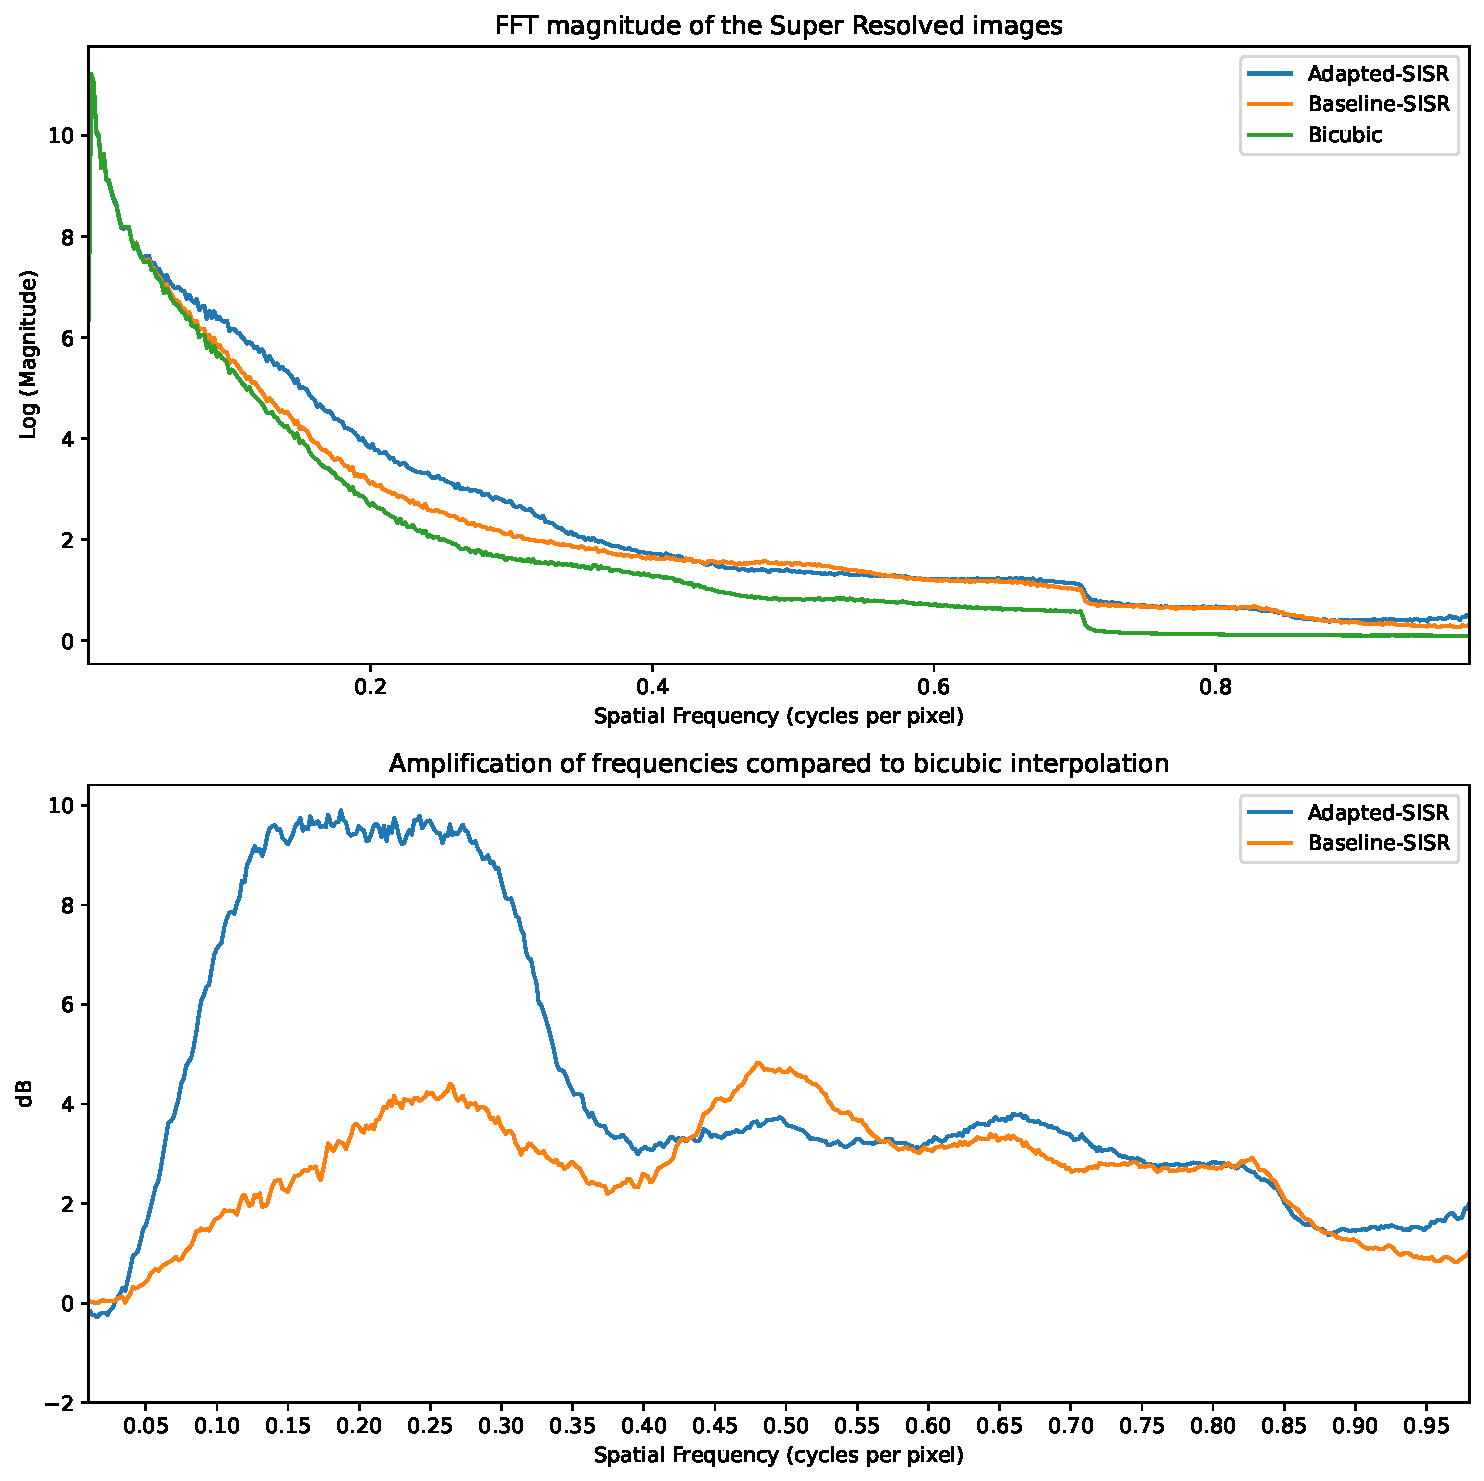
\includegraphics[scale=0.5]{Includes/6-target-fft-analysis.pdf}
                \caption{Frequency domain analysis of the super resolved images using different target domains vs. bicubic upsampling on the sample displayed on Fig. \ref{fig:6-target-fft-sample}}
                \label{fig:6-target-fft-analysis}
            \end{figure}


            


            
    
            \begin{figure}[ht!]
                \centering
                \includegraphics[scale=0.28]{Includes/6-target-gradient-analysis-image.pdf}
                \caption{Sample of adapted SISR}
                \label{fig:6-target-gradient-analysis-image}
            \end{figure}

            \begin{figure}[ht!]
                \centering
                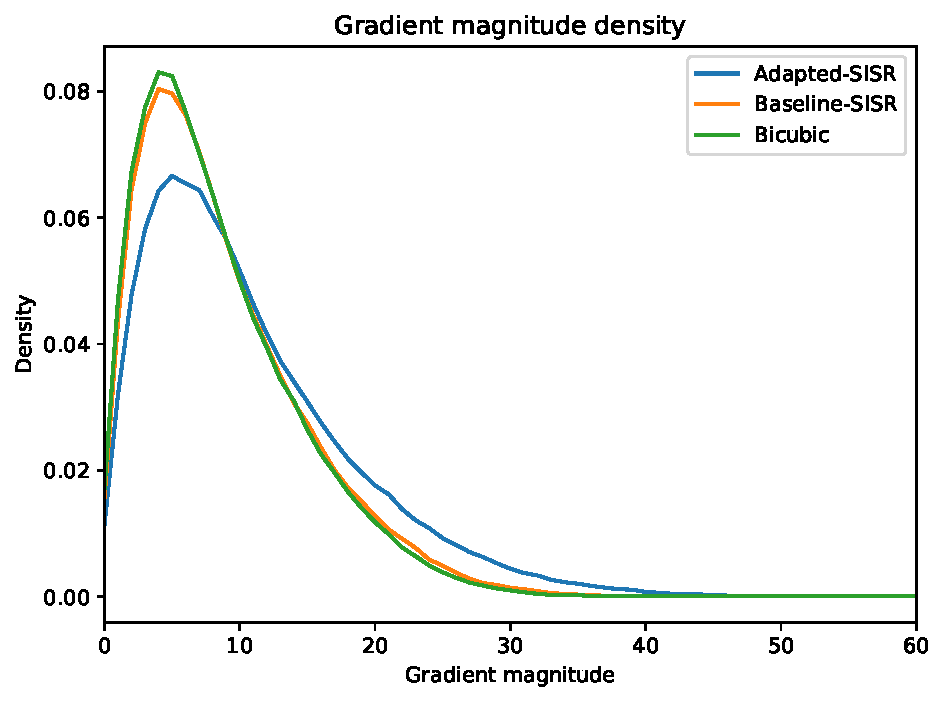
\includegraphics[scale=0.6]{Includes/6-target-gradient-analysis-histogram.pdf}
                \caption{Histogram of the gradient magnitude $|G|$ for the sample displayed in Fig. \ref{fig:6-target-gradient-analysis-image}}
                \label{fig:6-target-gradient-analysis-histogram}
            \end{figure}
        
        
% \breakpage
    